\section{IPM prototype Simulations}
\subsection{Project overview}
\begin{frame}
  \frametitle{Project overview}
  \begin{block}{Project in brief}
    Provide 5 pairs of IPMs for the superconducting part of the ESS accelerator.
    \begin{itemize}
      \item In-Kind collaboration between CEA/IRFU and ESS
      \item Around XX peoples involved
    \end{itemize}
  \end{block}
  \begin{block}{Project milestones}
    \begin{itemize}
      \item[2016] Kick-off meeting (April), beginning of my PhD (October)
      \item[2017] Preliminary Design Review (February), simulations, design and manufacturing
      \item[2018] \underline{Mainly beam tests and data analysis}
      \item[2019] Critical Design Review (March), design and manufacturing of final IPMs, end of my PhD (October)
      \item[2020] First IPM delivery, Handover
    \end{itemize}
  \end{block}
\end{frame}

\begin{frame}
  \frametitle{Requierements}
  \begin{columns}
    \begin{column}{0.45\textwidth}
      \begin{block}{Requierements on the measurement}
        ESS has specified some crucial requirements for the profilers.
        \begin{itemize}
          \item Measurement per pulse at nominal conditions
          \item Maximum error on the beam size $<\,10\,\%$
        \end{itemize}
      \end{block}
      \begin{block}{Other requierements}
        ESS has specified some crucial requirements for their diagnostics.
        \begin{itemize}
          \item Compliant to the use of superconductive cavities nearby
          \item Restricted environnement $\rightarrow$ the LWU
          \item The system must be sustained on a CF200 flange
        \end{itemize}
      \end{block}
    \end{column}
    \begin{column}{0.45\textwidth}
      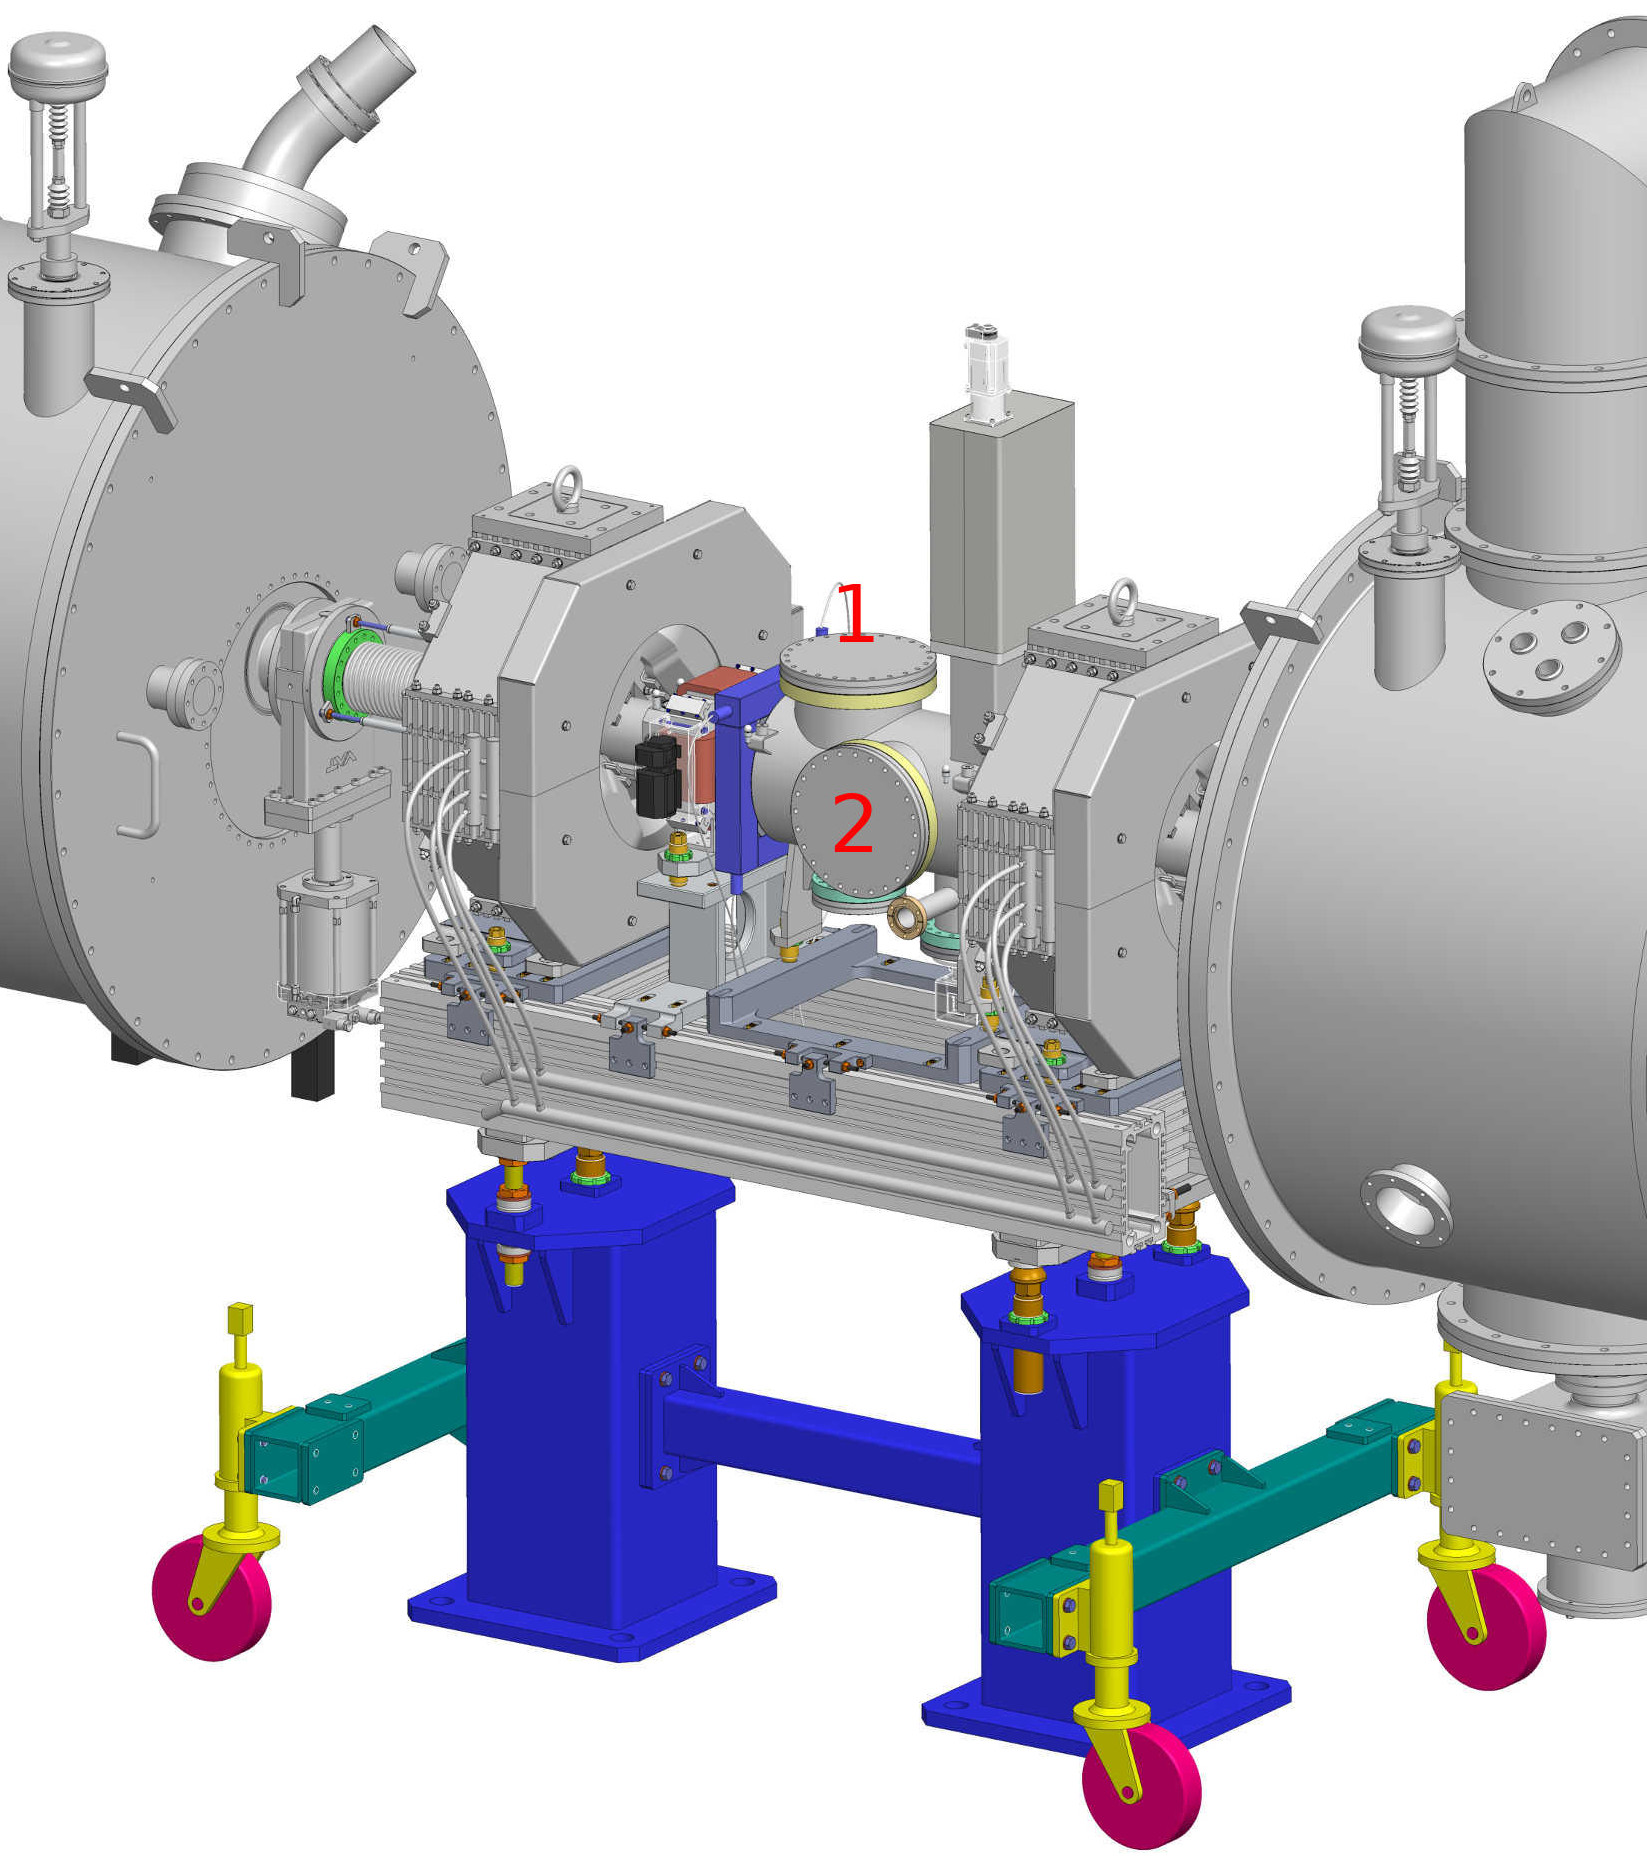
\includegraphics[width=\textwidth]{03_SIM/fig/fig016_LWU_Cryo4}
    \end{column}
  \end{columns}
\end{frame}

\begin{frame}
  \frametitle{IPM}
  \begin{columns}
    \begin{column}{0.45\textwidth}
      \begin{block}{Each step can be simulated}
        \begin{enumerate}
          \item Quantification of the "primary" ionization signal.
          \item Determination of the $e^-$/ion trajectories during the drift.
          \item The choice of an efficient readout technology.
        \end{enumerate}
      \end{block}
    \end{column}
    \begin{column}{0.45\textwidth}
      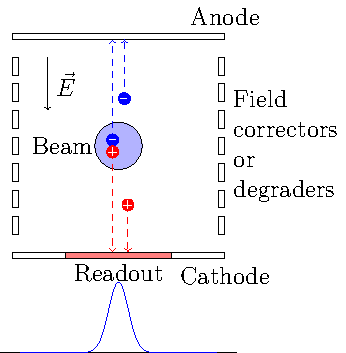
\includegraphics[width=\textwidth]{02_ESS/fig/fig000_IPM.pdf}
    \end{column}
  \end{columns}
\end{frame}

\subsection{Primary ionization signal}
\begin{frame}
  \frametitle{Primary ionization signal}
  \begin{block}{}
    \begin{itemize}
      \item
    \end{itemize}
  \end{block}
  \begin{alertblock}{}
    Huge dependance on vacuum parameters. Computation only gives an order of magnitude!
  \end{alertblock}
\end{frame}

\subsection{Profile distortion}
\begin{frame}
  \frametitle{Profile distortion}
  \begin{columns}
    \begin{column}{0.45\textwidth}
      \begin{block}{How it works}
        \begin{itemize}
          \item Quantification of the "primary" ionization signal.
          \item Determination of the $e^-$/ion trajectories during the drift.
          \item The choice of an efficient readout technology.
        \end{itemize}
      \end{block}
    \end{column}
    \begin{column}{0.45\textwidth}
      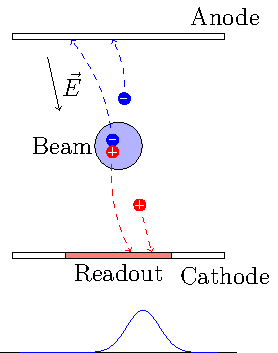
\includegraphics[width=\textwidth]{03_SIM/fig/fig000_IPM_distorsion.pdf}
    \end{column}
  \end{columns}
\end{frame}

\begin{frame}
  \frametitle{Field uniformity}
  \begin{itemize}
    \item IPM geometry itself
    \item The vacuum vessel that enclose the IPM
    \item Others devices in vacuum
  \end{itemize}
\end{frame}

\begin{frame}
  \frametitle{Field uniformity}
  \begin{itemize}
    \item IPM geometry itself
    \item The vacuum vessel that enclose the IPM
    \item IPM polarization
    \item Others devices in vacuum
  \end{itemize}
\end{frame}

\subsection{Space charge}
\begin{frame}
  \frametitle{Space charge}
  \begin{block}{Information}
    The space charge can be compensated:
    \begin{itemize}
      \item By adding a magnetic field about hundred $mT$ $\rightarrow$ impossible in our case
      \item By increasing the E field but limited by power supplies, sparks ...
    \end{itemize}
  \end{block}
\end{frame}

\begin{frame}
  \frametitle{Space charge}
  \begin{block}{}
    \begin{itemize}
      \item The space charge effect is more important for lower
      \item The space charge effect increase with beam current for lower
    \end{itemize}
  \end{block}

  \begin{alertblock}
    The measurement must be done with ion
  \end{alertblock}
\end{frame}

\subsection{Readout}
\begin{frame}
  \frametitle{Strip (multi electrode)}
  A moving particle induced a current on an electrode. The current is  thanks to Ramo-Sc theorem.
  \begin{itemize}
    \item Simple to implement
    \item Robust
  \end{itemize}
\end{frame}

\begin{frame}
  \frametitle{MCP}

  \begin{block}{Pro}
    \begin{itemize}
      \item Huge amplification
      \item Can be stacked
      \item High ion sensitivity
    \end{itemize}
  \end{block}

  \begin{block}{Prototype}
    We used single stage MCP from Hamamatsu and Photonis with P46 and P43 screen.
  \end{block}
\end{frame}

\begin{frame}
  \frametitle{Silicon}

  \begin{block}{Pro}
    \begin{itemize}
      \item Huge sensitivity with electron
      \item xx
    \end{itemize}
  \end{block}
  \begin{block}{Prototype}
    The CERN team kindly provided to us a FitPix kit (TimePix1) with ...
  \end{block}
\end{frame}

\begin{frame}
  \frametitle{Silicon}
  \begin{alertblock}{The use of ions}
    Silicon detector
    \begin{itemize}
      \item Multiple species in vacuum with various mass $\implies$ impossible to solve the ToA.
      \item Low penetration depth, may be not detected.
    \end{itemize}
  \end{alertblock}
\end{frame}